\section{Line encoding and decoding}
\label{sec:encoding_decoding}

Line encoders and decoders are essential components in the Physical OSI layer, which has also been described in section~\ref{Sub:Structure_Encoding}. Multiple ways of line encoding have been introduced over time and all have their own characteristics. Since many variants are still widely in use, this separate chapter has been written to provide more information on how important these techniques are. The process of encoding and decoding itself will be described in more detail but also other additions that play a role while encoding will be discussed. 

Each line encoding and decoding technique has it's own benefits while the drawbacks should also provide important knowledge. The presence of scramblers in modern ways of encoding will also be discussed. In short they are responsible for the prevention of DC offset by randomizing the data. Modern encoders are responsible for the addition of synchronization headers.

\subsection{8b/10b}
A fairly simple form of encoding which was developed by IBM in 1983. Each incoming byte will be translated into a constrained 10-bit binary.
%The maximum run length is 5 bits and the maximum digital sum variation is 6 bits. \\

The encoder actually consists of two components, a 5b/6b and a 3b/4b encoder. The last five bits of the incoming byte will be picked and placed at the start of the encoded byte. After these bits, an extra bit will be added. The remaining three first bits the incoming byte contained will follow with an extra bit added again.

Those so called extra bits are known as running disparity. These are variable bits to ensure the balance between ones and zeros is maintained. Otherwise DC unbalance can cause malfunctions in the system like explained in section~\ref{Sub:Structure_Encoding}~\cite{8b10b}.

The 5b/6b and 3b/4b encoders make use of separate tables to translate the original data bits to the accompanying encoded bits. This way of coding also provides the ability to transmit control symbols and characters to the receiver over the line.

8b/10b encoding is still widely in use despite multiple attempts have been made to develop better encoders. The reliability that comes with the encoder is why many protocols still use 8b/10b encoding. Also the absence of DC-imbalance is a huge advantage. This is possible because the used algorithm always balances the amount of ones and zeros. However the 20\% overhead that comes with it and increasing demands in transfer speeds cause protocols to slowly look for different variants of encoding.

Technologies using this way of encoding are among others DVI, HDMI, Gigabit Ethernet (SGMII), SATA, SAS, USB 3.0 and XAUI.


\subsection{64b/66b}
At the time of writing 8b/10b encoding is still widely used but the 20\% overhead is quickly becoming a bottleneck while transmitting data a high rates. Different and more efficient ways of encoding have been introduced and 64b/66b is one of them. It is immediately clear that this way up to eight bytes can be transmitted in one package while using a two-bit preamble. This way of encoding provides a better approach to prevent the earlier discussed quite large overhead, which in size went from 20\% to a decreased percentage of little over 3\%. Less bandwidth is wasted using this approach and more data can be transferred in the same time. Before transmitting, the data will be scrambled using a self synchronous scrambler with a 58-bit polynomial and eventually the receiver will unscramble the data~\cite{NIcoding}.

\begin{figure}[ht]
	\centering
	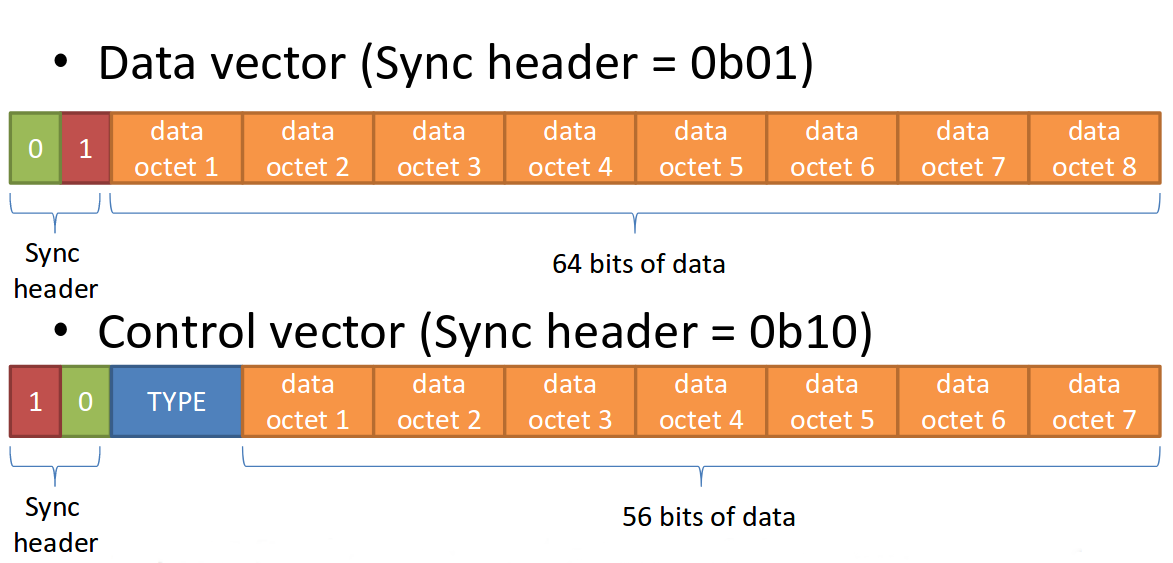
\includegraphics[width=0.7\textwidth]{6466header.png}	
	\caption{Headers used for 64b/66b encoding.}
	\label{fig:6466header}
\end{figure} 

In Figure~\ref{fig:6466header} two different data blocks are visible~\cite{6466header}. The upper one is just a block containing the eight bytes of data. The lower block contains the control commands. It consists of seven bytes and a two bit type indication. This structure could vary depending on the protocol but it gives a general overview of what the two types of encoded vectors/blocks look like.  

Technologies who adopted this way of encoding are for example 10/100 Gigabit Ethernet, InfiniBand and Thunderbolt.


\subsection{128b/130b - PCIe 3.0/4.0}
This builds further on the 64b/66b encoding but now with twice the payload. It doesn't make use of self-synchronous scrambler and uses a different scrambling polynomial. The two preamble bits still have the same functionality as the case with 64b/66b encoding. The encoding results in less overhead and more bandwidth can be used to transmit data bytes. 

This way of encoding is for example used in PCI Express 3.0 and 4.0 which can reach line rates up to respectively 8 and 16 Gbps~\cite{PCIE}.

\subsection{128b/132b - USB 3.1}
Very alike with the earlier discussed 128b/130b encoding but with four preamble bits instead of two. This way of encoding is primarily used by the USB 3.1 protocol. The preamble is still used to indicate whether the transmitted information is a block containing data or a block that contains control commands. The first two bits or the preamble are set to indicate a control block and the last two are used to indicate a block containing data.

The two extra bits in the preamble have been added to decrease the error-rate compared to earlier USB versions. The protocol will stay running if a single bit flips and can correct that flip. When two or more bits flip, the protocol will go to into recovery. Same would be the case with a single bit when the two preamble bits were used~\cite{USB3.1}.

\subsection{256b/257b - Fibrechannel}
This a way of encoding results in a very big packet of data to be transmitted. Four incoming 66 bit blocks are converted into a single 257 bit block. This is done by a of course removing some of the bits but without influencing the actual data and control commands. In Figure~\ref{fig:256257_data_header} a transmission packet containing exclusively data is visualized~\cite{256b/257b}.

\begin{figure}[ht]
	\centering
	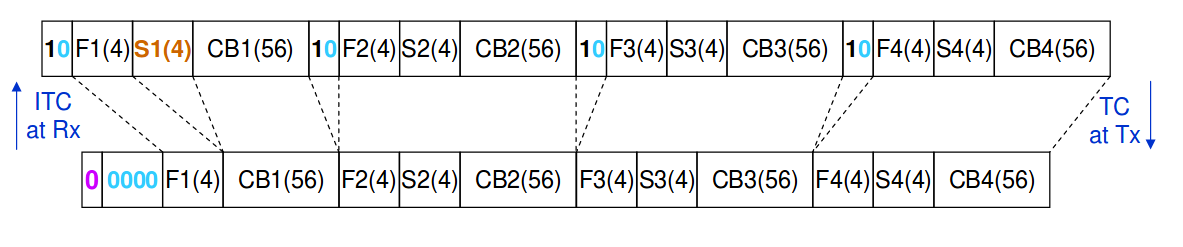
\includegraphics[width=0.7\textwidth]{256b257b.png}	
	\caption{The header of a 256b/257b transmission containing data.}
	\label{fig:256257_data_header}
\end{figure}

When four eight data byte blocks in a row have to be transmitted, it is fairly simple to put these in a single 257b block by removing all the preambles and putting a single preamble bit in front of the transmitted block. A one indicates that only data blocks are being transmitted and a zero indicated control block or a mix of data and control. Figure \ref{fig:256257_mixed_sheader} shows a transmission packet containing data and control blocks~\cite{256b/257b}.

\begin{figure}[ht]
	\centering
	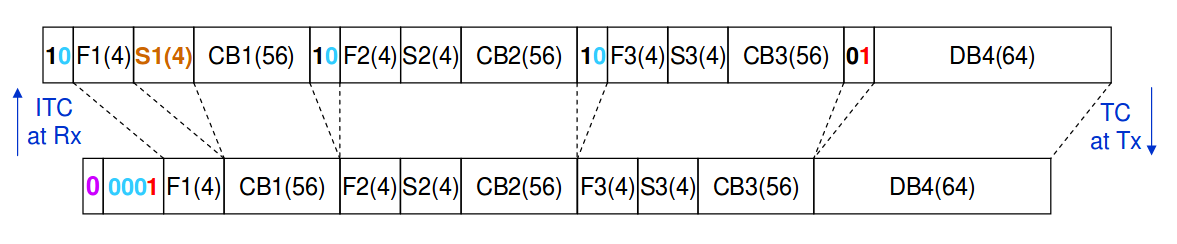
\includegraphics[width=0.7\textwidth]{256b257b2.png}	
	\caption{The header of a 256b/257b transmission with mixed blocks.}
	\label{fig:256257_mixed_sheader}
\end{figure}

When only control blocks or both variants are sent in a single block. The first bit will be zero and the following four bits will indicate which bytes are data or control commands. The first nibble of a command block will be removed to make room for the four additional bits. This way the block can be transmitted with less than 2\% overhead.

This way of encoding is used by FibreChannel in the 32G and 128G variants~\cite{FibreChannel_Encoding}.

\subsection{64b/67b - Interlaken/SerialLite}
\label{subsec:64b67b}
This is nearly identical to the structure used in 64b/66b encoding. The only difference is the addition of an extra bit to the preamble. While 64b/66b encoding completely depends on the scrambler to prevent DC base wandering, this way of encoding also has the ability to invert the data that will be transmitted. If this data has the tendency to excessively increase or decrease the line voltage, the data pack excluding the preamble can be inverted. This inversion is indicated using the additional bit which is referred to as the inversion bit. This makes the decoder clear whether the data is has been inverted and the data will always leave the decoder with it's original polarity.

Analysis has shown that the scrambler 64b/66b encoding trusts so much on, is not perfect and can still cause DC base wandering over time.  This is why the 64b/67b encoding has been developed. The only protocols using this way of encoding at the moment of writing are the Interlaken protocol~\cite{InterlakenProtocol} and Altera/IntelFPGA SerialLite~\cite{SerialLiteIII_MainPage}.

\subsection{Scramblers}
It should be taken in account that long streams of ones and zeros create a constant voltage. This could be a harmful phenomenon while synchronizing a communication system because there is a short on transition states. Several ways of encoding were developed to overcome this problem but nonetheless without success since they actually didn't solve the problem but provided workarounds. One of the workarounds was to limit the maximum length of a possible string only containing ones or zeros. Of course this wasn't a direct solution to the existing problem but it was the easiest way to get the transmission suited for long-distance communication.

A more appropriate solution was the so called scrambler. A scrambler randomizes the data input sequence in such way that it is nearly guaranteed there will be no long streams which only contain ones or zeros. After this scrambling the data is still recoverable with a descrambler that will be placed at the receiving side.\\
Unfortunately the scrambler cannot completely guarantee the prevention of such a long stream of ones and zeros but it will minimize the probability.

Implementing a scrambler provides even more benefits. Beside the prevention of a DC component it provides good error detection, good synchronization capability, eases clock recovery performance and offers the possibility to send data over long distances~\cite{scrambler}. \\
A physical scrambler is realized by implementing a parallel register and several XOR gates.

\newpage
